\documentclass[11pt]{article}

\usepackage[utf8]{inputenc}
\usepackage[danish]{babel}
\usepackage[T1]{fontenc}
\usepackage{float}
\usepackage{fancyhdr}
\usepackage{amsmath}
\usepackage{color}
\usepackage{graphicx}
\usepackage{lastpage}
\usepackage{enumitem}
\usepackage{wrapfig}
\usepackage[a4paper, top = 1in, bottom = 1in, left=1in,right=1in]{geometry}
\usepackage[hidelinks]{hyperref}

\newcommand{\tabitem}{~~\llap{\textbullet}~~}

\newcommand{\resumeSubheading}[4]{
  \noindent\begin{tabular*}{0.98\textwidth}[t]{l@{\extracolsep{\fill}}r}
    \noindent \textbf{#1} & #2 \\ \vspace{-3pt} 
    \noindent \textit{\small#3} & \textit{\small #4} 
  \end{tabular*}\vspace{7pt}
}

\newcommand{\listitem}[2]{
  {\small{\tabitem{#1}}} & {\small\tabitem{#2}}\\
}

\begin{document}
\begin{center}
  \textbf{\huge{\scshape{Peter Heilbo Ratgen}}}\\ 
  \vspace{0.2cm}
  \small 31330916 $|$
  \href{mailto:peter@pratgen.dk}{\underline{peter@pratgen.dk}} $|$
  \href{https://github.com/PeterRatgen }{\underline{github}} $|$
  \href{https://pratgen.dk}{\underline{pratgen.dk}} $|$
  \href{https://www.linkedin.com/in/peter-ratgen-a1236529/}{\underline{linkedin}}
\end{center}

\noindent\large{\scshape{About - Personal}} \newline
\noindent{\rule[0.3cm]{\textwidth}{0.4pt}}

  \begin{wrapfigure}{R}{0.2\textwidth}
    \vspace{-0.7cm}
    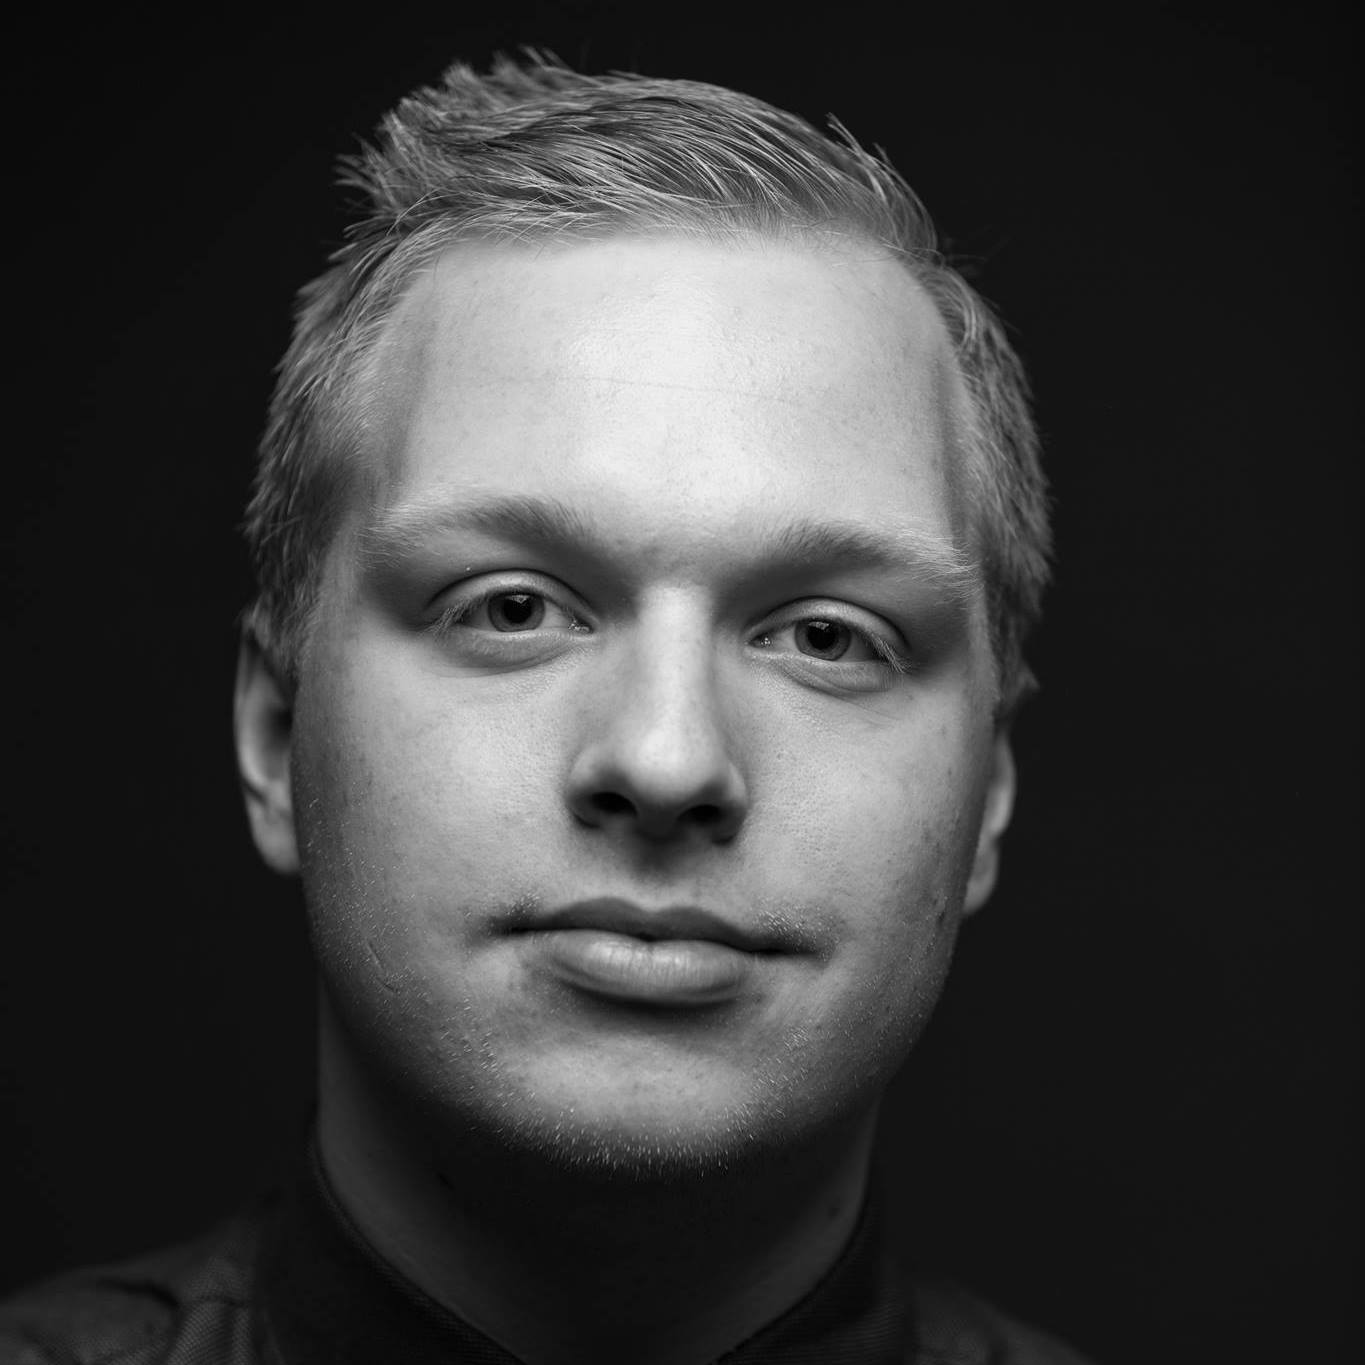
\includegraphics[width=0.2\textwidth]{./okay.jpg}
  \end{wrapfigure}
{\normalsize Software Engineering student, former Computer Science Student, based
  in Odense, 22 years old. I am driven, and love to dive deep into projects. I
  am passionate about learning new usable skills, and increasing productivity
  using new tools. I am especially interested in back-end web-development, and
  working with Linux. 
  
  
}

\vspace{0.3cm}
\noindent\large{\scshape{Education}} \newline
\noindent{\rule[0.3cm]{\textwidth}{0.4pt}}

\resumeSubheading{University of Southern Denmark}{}{Software Engineering}{Sep.
2020 -- Jun. 2022}\\\vspace{0.25cm}
{\indent\small Currently taking these courses:}
  \vspace{-0.3cm}
  {\small 
  \begin{itemize}
  \setlength{\itemsep}{-1pt}
    \item Statistical Data Analysis
    \item Human Computer Interaction
    \item Semesterproject: Interactive Distributed Software Systems
      \subitem Creating a media player using HTML and JavaScript, working with
      docker images and kubernetes. Interacting with other teams through APIs.
\end{itemize}} \vspace{0.3cm}


\resumeSubheading{University of Southern Denmark}{}{Computer Science}{Sep. 2017
-- Mar. 2020}\\\vspace{0.25cm} 
{\indent\small Completed 130 ECTS towards a Computer Science bachelors degree,
completed courses in:}
  \vspace{-0.3cm}
  {\footnotesize 
  \begin{itemize}
  \setlength{\itemsep}{-1pt}
    \item Discrete Methods for Computer Science
    \item Introduction to Programming
    \item Algorithms and Data Structures
    \item Database Design and Programming
    \item Concurrent Programming
    \item Networks and Security
    \item Computer architecture and system programming
    \item Linear algebra with applications
    \item Operating Systems
    \item Data mining and machine learning
    \item Formal Languages and Data Processing
    \item Software Engineering
\end{itemize}}
\vspace{0.3cm}

\resumeSubheading{Odense Tekniske Gymnasium}{}{Higher Technical
Examination (HTX)}{Aug. 2014 -- Jun. 2017}
{\small \begin{itemize}\vspace{-0.25cm}
  \setlength{\itemsep}{-1pt}
  \item Specialized study area: Communication/IT A, Design B
    \subitem Worked with graphic design, and communication in general.

  \item Technical science: Technical Sciences A, Electricity
    \subitem\footnotesize Worked with the PIC microcontroller.
\end{itemize}
} \vspace{0.5cm}

\newpage
\noindent\large{\scshape{Acquired Skills}} \newline
\noindent{\rule[0.3cm]{\textwidth}{0.4pt}}


  \noindent\begin{tabular*}{0.62\paperwidth}[t]{l@{\extracolsep{\fill}}l}
    \textbf{Languages} & \textbf{Tools} \\ 
    \listitem{Python}{Vim}
    \listitem{Java}{Git}
    \listitem{Lua}{Command Line (Linux/Mac)}
    \listitem{JavaScript}{Bash}
    \listitem{Postgres SQL}{Docker}
    \listitem{HTML/CSS}{Kubernetes}
    \listitem{C}{Apache}
                       & \small{\tabitem{LaTeX}} \\
                      & \\
    \textbf{Misc. tools} & \textbf{Languages}  \\
    \small{\tabitem{Adobe Photoshop}} & \small{\tabitem{Danish, primary}} \\
    \small{\tabitem{Adobe Illustrator}} & \small{\tabitem{English}}\\
    \small{\tabitem{Adobe InDesign}} & \small{\indent Written and spoken} \\

  \end{tabular*}\vspace{7pt}
\vspace{0.5cm}

\noindent\large{\scshape{Previous Jobs}} \newline
\noindent{\rule[0.3cm]{\textwidth}{0.4pt}}
\resumeSubheading{Boogies}{}{Cleaner}{Sep. 2018 -- Present}
\vspace{0.3cm}

\resumeSubheading{Design Danmark}{}{Graphic Designer}{Feb. 2016 -- May 2017}\\
\indent{\small Created menu design for prominent café in Odense, and implemented it in
Adobe InDesign. Created logos for clients to consider in Adobe Illustrator.}
\vspace{0.3cm}

\resumeSubheading{Dreamsprit Photography}{}{Photo Editor/Co-owner}{Mar. 2015 --
Jun. 2017}\\
\indent{\small Photography project in free time, editing photos shot in Adobe
Photoshop, miscellaneous graphical tasks}
\end{document}
